% !TEX TS-program = Xelatex
% !TEX encoding = UTF-8 Unicode

\documentclass[UTF8]{ctexart}
\usepackage{amsmath}
\usepackage[bottom]{footmisc}
\usepackage{geometry}
\usepackage{graphicx}
\usepackage{figsize}
\usepackage[separate-uncertainty = true,per-mode=symbol]{siunitx}
\usepackage{tabu}
\usepackage{wasysym}
\geometry{left=0.7in,right=0.7in,bottom=0.7in,top=0.7in}

\title{实验二十:夫琅禾费衍射}
\author{朱寅杰 1600017721}
\date{2017年12月8日}

\begin{document}
\maketitle
根据夫琅禾费衍射的定量计算结果,有
\[
I=I_0(\frac{\sin u}{u})^2(\frac{\sin{N\beta}}{N\beta})^2,u=(x-x_0)\frac{\pi a}{\lambda z},\beta=(x-x_0)\frac{\pi d}{\lambda z}
\]
其中$I$为在$x$处的光强,$a$为缝宽,$d$为缝间距,$N=1,2,3,4...$为缝的数目,$z$为缝到接收面的距离(做了$z\gg x$的近似),$\lambda$为激光波长。

实验时使用波长$\lambda=\SI{632.8}{\nm}$的氦氖激光器作为光源,在光学平台上搭出夫琅禾费衍射的光路。使用硅光电二极管传感器配合一台步进电机测量接受面上不同位置的光强,当$x$每改变\SI{0.005}{\mm}时记录一个$I$的数据。由衍射所得的$I-x$关系,从上面的公式中拟合出$\frac{\pi a}{\lambda z}$与$\frac{\pi d}{\lambda z}$的数值,从而得到缝宽和缝间距的测量结果。

对于单缝衍射,$N=1$。用固定在平台上的钢尺测量出$z=\SI{94.10}{\cm}-\SI{28.20}{\cm}+\SI{4}{\mm}=\SI{66.3}{\cm}$(将传感器与缝的位置坐标相减,并加上传感器实际位置的一个修正)。$z$的不确定度就按\SI{1}{\mm}估计吧。使用Origin软件对该数据进行拟合,通过内置的迭代方法计算出一个所谓的相关系数$r^2=0.99977$,以及各参量$I_0=\num{3243.6(6)},x_0=\SI{18.8967(3)}{\mm}$,
\[\frac{\pi a}{\lambda z}=\SI{0.9383(2)}{\per\mm}\]
于是可以计算出缝宽$a=\SI{1.253(2)e-4}{\m}$

对于双缝衍射,$N=2$。用固定在平台上的钢尺测量出$z=\SI{94.10}{\cm}-\SI{37.80}{\cm}+\SI{4}{\mm}=\SI{56.7}{\cm}$。$z$的不确定度按\SI{1}{\mm}估计。使用Origin软件对光强数据进行拟合,通过内置的迭代方法计算出一个所谓的相关系数$r^2=0.99108$,以及参量$I_0=\num{900.6(8)},x_0=\SI{32.3569(9)}{\mm}$,
\[\frac{\pi a}{\lambda z}=\SI{0.4049(3)}{\per\mm},\frac{\pi d}{\lambda z}=\SI{.7652(3)}{\per\mm}\]
于是可以计算出缝宽$a=\SI{4.624(9)e-5}{\m}$,缝间距$b=\SI{8.74(2)e-5}{\m}$。

对于四缝衍射,$N=4$。用固定在平台上的钢尺测量出$z=\SI{94.10}{\cm}-\SI{28.58}{\cm}+\SI{4}{\mm}=\SI{65.92}{\cm}$。$z$的不确定度按\SI{1}{\mm}估计。使用Origin软件对光强数据进行拟合,通过内置的迭代方法计算出一个相关系数$r^2=0.98952$,以及各参量$I_0=\num{237.6(3)},x_0=\SI{16.5486(6)}{\mm}$,
\[\frac{\pi a}{\lambda z}=\SI{0.3017(4)}{\per\mm},\frac{\pi d}{\lambda z}=\SI{.6978(2)}{\per\mm},\]
于是可以计算出缝宽$a=\SI{4.006(6)e-5}{\m}$,缝间距$b=\SI{9.265(14)e-5}{\m}$。
\paragraph{说明}
单缝、双缝和四缝的$I-x$关系的拟合经软件作图绘制于附页中。可以看到单缝与四缝的拟合较好,从拟合曲线中计算出的缝宽等参数应当是比较准确的;而双缝的曲线拟合出来并不理想(可以看到在几个高级条纹中峰谷都没有对齐,因此对于缝宽的拟合甚至可以说是相当失败的……尝试过调整软件计算拟合参数时的迭代起点以期能得到最优解而非这样的次优解,但并没有收到太好的效果。)如果直接从图上凭肉眼找包络的位置的话,算出的缝宽约为\SI{3.9e-5}{\m},这个数值应该可能为准确一些。

这就自然暴露出一个问题,就是软件给出的各拟合参量的标准差(也就是列于计算结果中的那些)并不能反映出它们实际的不确定度。这个标准差应该是通过$r^2$之类的参数,通过类似于之前学过的$\sqrt{(1/r^2-1}/(N-2)}$的算法得到的。由于这里的$N$十分巨大,因此这个标准差自然就会非常小。

经同学提醒

附图中还有十张观察不同孔(或是丝)的衍射花样。从中大概能直观感受“夫琅禾费衍射花样是衍射物的傅立叶变换”的含义。最明白的规律好比有圆孔的衍射花样是“各向同性”地旋转对称的,而方孔的衍射花样

\begin{figure}
\centering
\SetFigLayout{3}{1}
\subfigure[单缝衍射的$I-x$图线与拟合曲线。]{\includegraphics[width=\linewidth]{1slit.eps}} \\
\subfigure[双缝衍射的$I-x$图线与拟合曲线。]{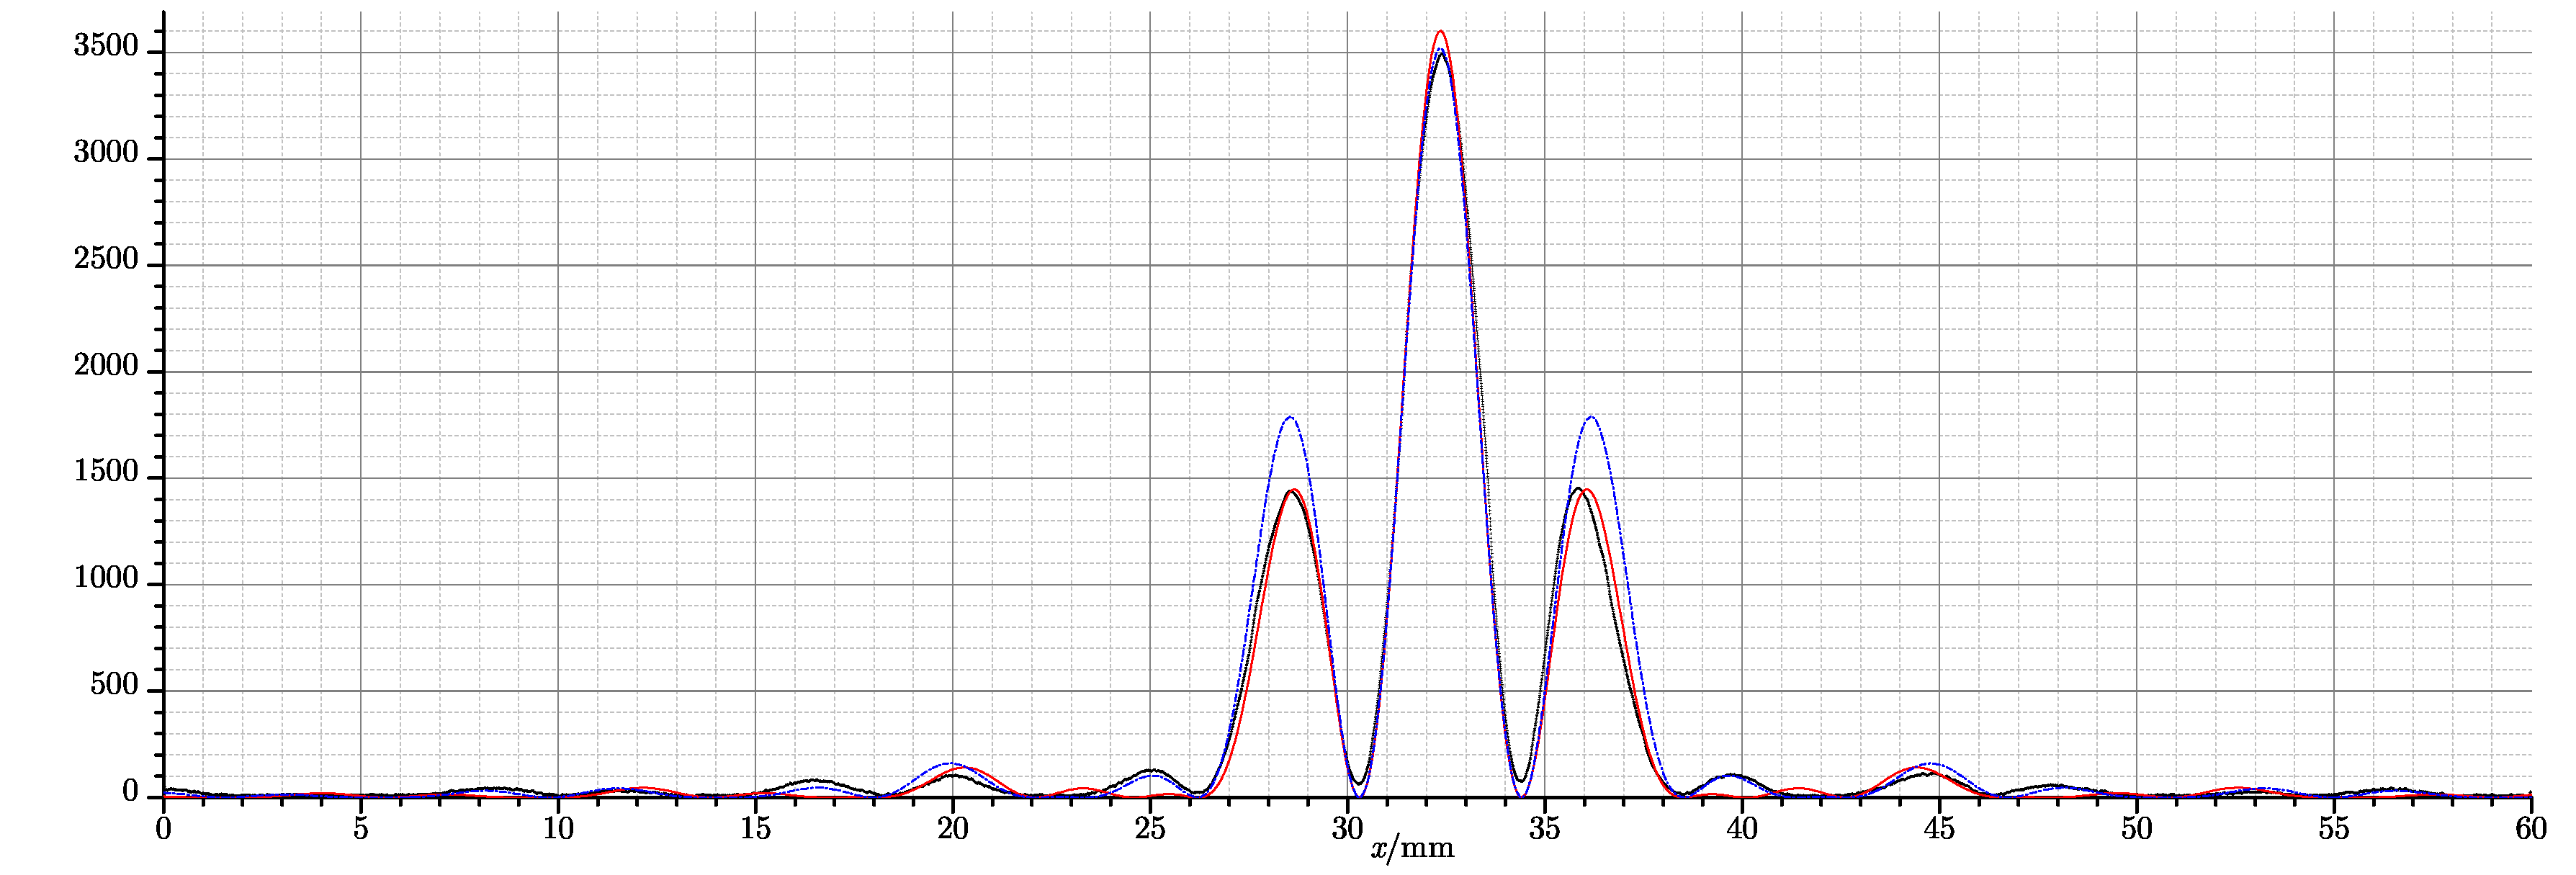
\includegraphics[width=\linewidth]{2slit.eps}} \\
\subfigure[四缝衍射的$I-x$图线与拟合曲线。]{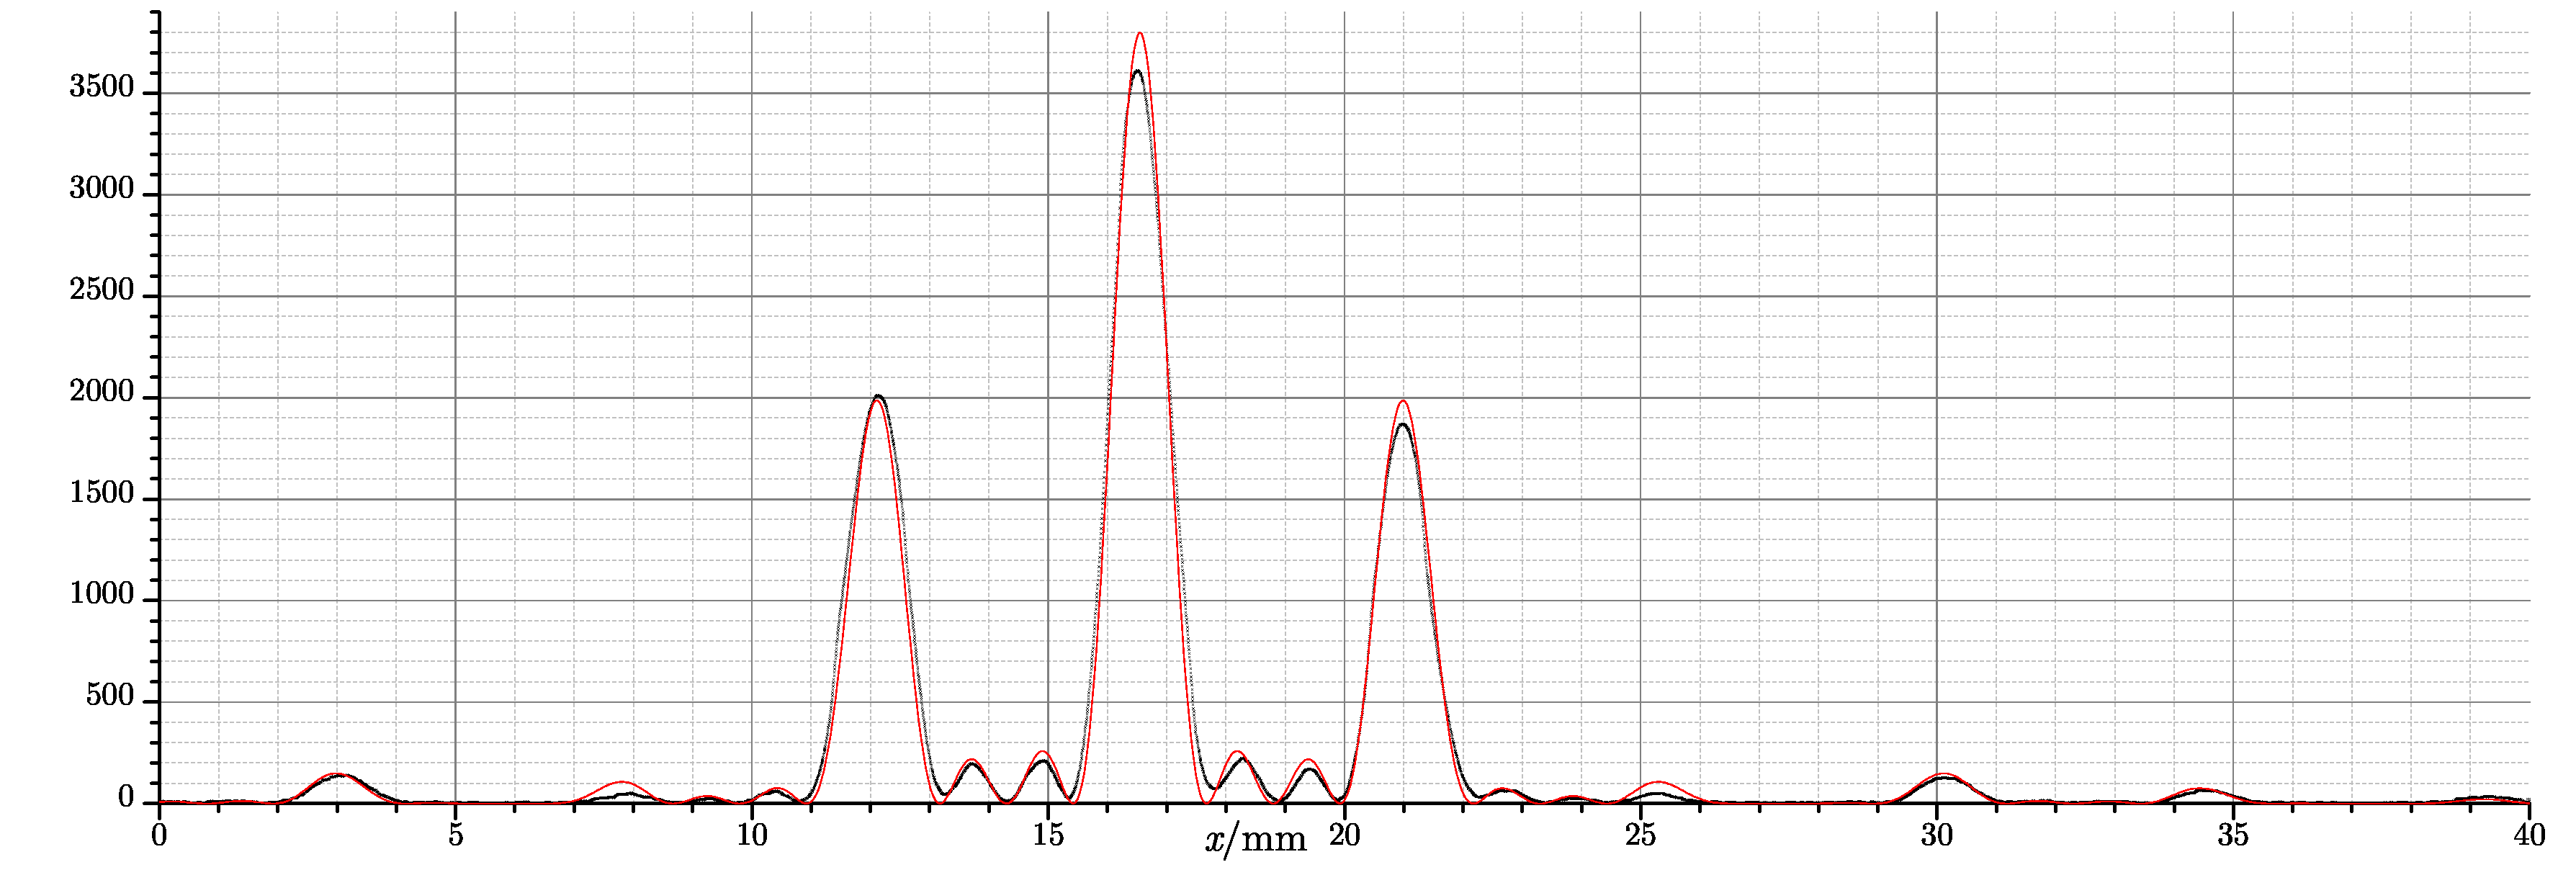
\includegraphics[width=\linewidth]{4slit.eps}} \\
\end{figure}
\begin{figure}
\centering
\SetFigLayout{5}{1}
\subfigure[衍射物为单丝。]{\includegraphics[width=\linewidth]{1.jpg}} \\
\subfigure[衍射物为双丝。]{\includegraphics[width=\linewidth]{2.jpg}} \\
\subfigure[衍射物为三丝。]{\includegraphics[width=\linewidth]{3.jpg}} \\
\subfigure[衍射物为四丝。]{\includegraphics[width=\linewidth]{4.jpg}} \\
\subfigure[衍射物为五丝。]{\includegraphics[width=\linewidth]{5.jpg}} \\
\end{figure}

\begin{figure}
\centering
\SetFigLayout{3}{2}
\subfigure[等边三角形孔的衍射花样。]{\includegraphics[width=0.45\linewidth]{db.jpg}}\hfill
\subfigure[等腰三角形孔的衍射花样。]{\includegraphics[width=0.45\linewidth]{dy.jpg}} \\
\subfigure[方孔方阵的衍射花样。]{\includegraphics[width=0.45\linewidth]{ff.jpg}}\hfill
\subfigure[密堆方孔的衍射花样。]{\includegraphics[width=0.45\linewidth]{yf.jpg}} \\
\subfigure[密堆圆孔的衍射花样。]{\includegraphics[width=0.45\linewidth]{ym.jpg}} \hfill\\
\end{figure}

\end{document}